\documentclass[../main/Notes.tex]{subfiles}
\begin{document}

\section[Signal Detection Theory III]{Signal Detection Theory III \iftoggle{showdates}{\small{\textit{2014-06-20}}}{}}
% quick workaround due to file loss, not the wrong chapter numbering
%\includepdf[pages={-},addtotoc={1,section,1,Signal Detection Theory III,signaldettheoryIII}]{../chapters/2014-06-20vorlaeufig.pdf}

\subsection{From YN to 2AFC}
In comparison to simple Yes-No-task there exists an alternative task design which is the 2-Alternative-Forced-Choice-task. In each trial the subject is presented with two intervals with a light stimulus in one of it, therefore there are two "stimulations" $X_{1}$,$X_{2}$. The probabilities for this experiment are given in the following.\\
\begin{tabular}{l l l}
\begin{tabular}{l}
$\left( X_{1}|S=1\right)\sim N\left( \Delta \mu , \sigma^{2}\right)$ \tikz[remember picture] \node[coordinate,yshift=0.5em, xshift=9.5cm] (n1) {}; \\ \\ \\ \smallskip \\
$\left( X_{2}|S=1\right)\sim N\left( 0 , \sigma^{2}\right)$ \tikz[remember picture] \node[coordinate] (n2) {};
\end{tabular} & 
\begin{tabular}{l}
\small - The probability distribution for a stimulation in the first\\ \small interval given that the signal was in the first interval \\  \\ \\ \\
\end{tabular} &
\begin{tikzpicture}[overlay,remember picture]
      \path (n2) -| node[coordinate] (n3) {} (n1);
      \draw[thick,decorate,decoration={brace,amplitude=3pt}]
            (n1) -- (n3) node[midway, right=4pt] {\small equal variance signal};
  \end{tikzpicture}
\\ \smallskip \\
\begin{tabular}{l}
% \\  \\
$\left( X_{1}|S=2\right)\sim N\left( 0 , \sigma^{2}\right)$\\ \\ \\ \smallskip \\
$\left( X_{2}|S=2\right)\sim N\left( \Delta \mu , \sigma^{2}\right)$
\end{tabular} &
\begin{tabular}{l}
\begin{tikzpicture}[scale=0.5]
\begin{axis}[every axis plot post/.append style={mark=none, domain=-4:4, samples=50, smooth}, 
    axis x line*=bottom, axis y line*=left, ticks=none, ylabel={S=1}, enlargelimits=upper, name=gauss]
    \addplot [red, ultra thick]    {gauss(-2,0.5)};% node[pos=0.4,  anchor=east] {$\sigma=0.5$};
    \addplot [green, ultra thick]  {gauss(2.5,0.5)};%   node[pos=0.6,  anchor=west] {$\sigma=1$};
    \node [above] at (axis cs:  -2, 0) {$0$};
\node [above] at (axis cs:  2.5, 0) {$\Delta \mu$};
  \end{axis}
  \draw [black,decorate,decoration={brace,amplitude=5pt,mirror},xshift=0.4pt,yshift=-0.4pt](0,0) -- (3,0) node[black,midway,yshift=-0.6cm] {\footnotesize $2^{nd}interval$};
\draw [black,decorate,decoration={brace,amplitude=5pt,mirror},xshift=0.4pt,yshift=-0.4pt](3.5,0) -- (6.5,0) node[black,midway,yshift=-0.6cm] {\footnotesize $1^{st}interval$};  \end{tikzpicture}
  \begin{tikzpicture}[scale=0.5]
\begin{axis}[every axis plot post/.append style={mark=none, domain=-4:4, samples=50, smooth}, 
    axis x line*=bottom, axis y line*=left, ticks=none, ylabel={S=2}, enlargelimits=upper, name=gauss]
    \addplot [red, ultra thick]    {gauss(-2,0.5)};% node[pos=0.4,  anchor=east] {$\sigma=0.5$};
    \addplot [green, ultra thick]  {gauss(2.5,0.5)};%   node[pos=0.6,  anchor=west] {$\sigma=1$};
    \node [above] at (axis cs:  -2, 0) {$0$};
\node [above] at (axis cs:  2.5, 0) {$\Delta \mu$};
  \end{axis}
  \draw [black,decorate,decoration={brace,amplitude=5pt,mirror},xshift=0.4pt,yshift=-0.4pt](0,0) -- (3,0) node[black,midway,yshift=-0.6cm] {\footnotesize $1^{st}interval$};
\draw [black,decorate,decoration={brace,amplitude=5pt,mirror},xshift=0.4pt,yshift=-0.4pt](3.5,0) -- (6.5,0) node[black,midway,yshift=-0.6cm] {\footnotesize $2^{nd}interval$};
\end{tikzpicture} 
\end{tabular} &
\end{tabular}


\begin{tikzpicture}[scale=0.9]
\begin{axis}[hide axis, domain=-4:4, y domain=-4:4, x=4.75cm, y=4.75cm, ticks=none ]
\end{axis}
\draw (4.7,1) circle (1cm);
\draw (4.7,1) circle (0.8cm);
\draw (4.7,1) circle (0.6cm);
\draw (4.7,1) circle (0.4cm);
\draw (4.7,1) circle (0.2cm);
\draw (1,4.7) circle (1cm);
\draw (1,4.7) circle (0.8cm);
\draw (1,4.7) circle (0.6cm);
\draw (1,4.7) circle (0.4cm);
\draw (1,4.7) circle (0.2cm);
\node [left] at (1, 3) {$X_{2}$};
\node [above] at (3, 0.5) {$X_{1}$};
\node [above] at (4.7, 2) {S=1};
\node [right] at (2 ,4.7) {S=2};
\node [left] at (5.25, 5.25) {\footnotesize decision boundary};
\draw[->, thick] (0, 1) -- (6, 1);
\draw[->, thick] (1, 0) -- (1, 6);
\draw (1, 4.7) -- (2,5.7);
\draw (4.7, 1) -- (5.7,2);
\begin{axis}[hide axis, yshift=0cm, every axis plot post/.append style={mark=none, domain=-4:5.75, samples=50, smooth}, 
    axis x line*=bottom, axis y line*=left, ticks=none, enlargelimits=upper,rotate=315, x=0.75cm, y=1.25cm]
\addplot [yellow, fill=yellow, fill opacity=0.4]  {gauss(-2.14,0.5)};
\end{axis}
\begin{axis}[hide axis,xshift=0.5cm,yshift=-0.5cm, every axis plot post/.append style={mark=none, domain=-5.5:4.25, samples=50, smooth}, 
    axis x line*=bottom, axis y line*=left, ticks=none, enlargelimits=upper,rotate=315, x=0.75cm, y=1.25cm ] %ticks=none,  
\addplot [yellow, fill=yellow, fill opacity=0.4]  {gauss(2.425,0.5)};
\end{axis}
\draw [fill=yellow , fill opacity=0.2] (4.7,1) -- (1,4.7) -- (1,1) circle;
\draw (1,1) -- (5.25,5.25);
\end{tikzpicture}\\
\begin{minipage}[t][3.25cm][t]{9.25cm}
Distance of the $\Delta \mu$: $\Delta \mu_{2AFC} = \sqrt{2}\Delta\mu
$\\
Best strategy for the best performance in 2AFC:
\begin{itemize}
\item Say 1 if $X_{1} > X_{2}$
\item Say 2 if $X_{2} \geq X_{1}$
\end{itemize}
$\Rightarrow \Delta X= X_{2}-X_{1} \stackrel{!}{>}0$
\end{minipage}
\fbox{
\begin{minipage}[t][0.7cm][t]{6cm}
d' = Detection Performance in YN-task\\
= signal-to-noise-ratio
\end{minipage}
}\\
\bigskip
\\
\begin{minipage}[t][3cm][t]{9.25cm}
What is the distribution of $\Delta X$?

$\left(\Delta X | S = 1\right) \sim N\left( -\Delta \mu , 2\sigma^{2}\right)$

$\left(\Delta X | S = 2\right) \sim N\left( \Delta \mu , \sigma^{2} + \left(\left( -1 \right)\sigma\right)^{2}\right) = N \left( \Delta \mu , 2\sigma^{2}\right)$
\end{minipage} 
\begin{minipage}[t][3cm][t]{6cm}
Helpful rules:

$X_{1},X_{2}$ are normal N

$X_{1} \sim N\left(\mu_{1} , \sigma_{1}^{2}\right)$

$X_{2} \sim N\left(\mu_{2} , \sigma_{2}^{2}\right)$

$aX_{1} \sim N\left(a\mu_{1} , \left(a\sigma_{1}\right)^{2}\right)$

$X_{1} + X_{2} \sim N \left( \mu_{1} + \mu_{2}, \sigma_{1}^{2} + \sigma_{2}^{2} \right)$
\end{minipage}
\\
\begin{minipage}[b][3cm][t]{3.5cm}
\begin{tikzpicture}[scale=0.5]
\begin{axis}[every axis plot post/.append style={mark=none, domain=-4:4, samples=50, smooth}, 
    axis x line*=bottom, axis y line*=left, ticks=none, enlargelimits=upper, name=gauss]
    \addplot [red, ultra thick]    {gauss(-2,0.5)};% node[pos=0.4,  anchor=east] {$\sigma=0.5$};
    \addplot [green, ultra thick]  {gauss(2.5,0.5)};%   node[pos=0.6,  anchor=west] {$\sigma=1$};
    \node [above] at (axis cs:  -2, 0) {$-\Delta\mu$};
\node [above] at (axis cs:  2.5, 0) {$\Delta \mu$};
\node [above] at (axis cs:  -2, 0.8) {S=1};
  \node [above] at (axis cs:  2.5, 0.8) {S=2};
  \end{axis}
\end{tikzpicture} 
\end{minipage}
\begin{minipage}[b][3.5cm][t]{8cm}
\begin{align*}
& & \Delta ~~~\mu_{2AFC} & = \sqrt{2}\Delta\mu ~~~|:\sigma & &\\
& & \Leftrightarrow d'_{2AFC} & = \sqrt{2}d' & & \\
& & \frac{\Delta\mu_{2AFC}}{\sigma} & = \frac{2\Delta\mu}{\sqrt{2}\sigma} = \sqrt{2}d' & & \\
& & d'_{2AFC} & = \frac{2d'}{\sqrt{2}\sigma} = \sqrt{2}d' ~~~\left(\text{same result as in the geometric solution}\right) & &
\end{align*}
\end{minipage}
\subsection{Cue Combination}
Ernst \& Banks (2002) - Visuo-haptic cue combination
\begin{itemize}
\item Judge the size of a bar when you can see and feel it
\item You get two measurements of s
\begin{itemize}
\item $V \sim N\left(s,\sigma_{V}^{2}\right)$
\item $H \sim N\left(s,\sigma_{H}^{2}\right)$
\end{itemize}
\end{itemize}
\bigskip
\vspace{3.75cm}
\begin{tikzpicture}[overlay]
\begin{axis}[scale=0.75, every axis plot post/.append style={mark=none, domain=-2.25:4, samples=50, smooth}, 
    axis x line*=bottom, axis y line*=left, ticks=none, enlargelimits=upper, name=gauss]
    \addplot [red, ultra thick]    {gauss(0,0.5)};% node[pos=0.4,  anchor=east] {$\sigma=0.5$};
    \node [above] at (axis cs:  0, 0) {$s$};
\node [above] at (axis cs:  1.47, 0.7) {\footnotesize Haptics};
  \end{axis}
  \begin{axis}[scale=0.5, every axis plot post/.append style={mark=none, domain=-4.56:4, samples=50, smooth}, 
    axis x line*=bottom, axis y line*=left, ticks=none, enlargelimits=upper, name=gauss]
    \addplot [green, ultra thick]  {gauss(0,0.5)};%   node[pos=0.6,  anchor=west] {$\sigma=1$};
    \node [right] at (axis cs:  1.37, 0.77) {\footnotesize Vision};
  \end{axis}
\draw (1.8,2.375) -- (2.25,2.5);
\draw (1.9,3.575) -- (2.25,3.7);
\end{tikzpicture} \\
%\bigskip
\\
What should be my estimate $\hat{s}$ of $s$?
\smallskip
\\
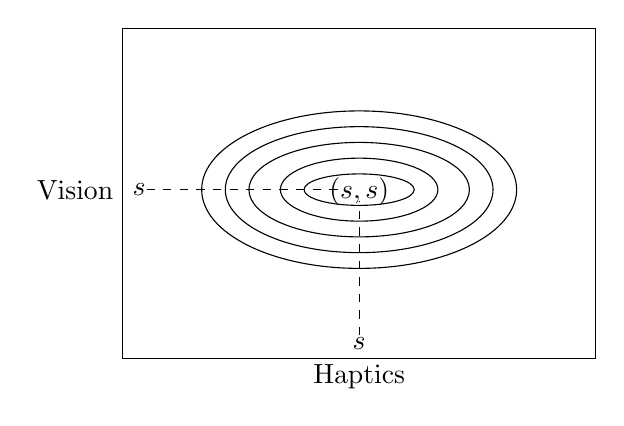
\begin{tikzpicture}
\begin{axis}[domain=-0none4:4, y domain=-4:4, x=5cm, y=3.5cm, ticks=none]
\end{axis}
\draw (3,2.15) ellipse (2cm and 1cm);
\draw (3,2.15) ellipse (1.7cm and 0.8cm);
\draw (3,2.15) ellipse (1.4cm and 0.6cm);
\draw (3,2.15) ellipse (1cm and 0.4cm);
\draw (3,2.15) ellipse (0.7cm and 0.2cm);
\node [above] at (3, 1.825) {$(s,s)$};
\node [right] at (0, 2.15) {$s$};
\node [left] at (0, 2.15) {Vision};
\node [above] at (3, 0) {$s$};
\node [above] at (3, -0.5) {Haptics};
\draw [dashed] (0.3, 2.15) -- (2.8, 2.15);
\draw [dashed] (3, 0.3) -- (3, 2);
\end{tikzpicture}\\
$p\left(V=v;H=h|s\right)=\frac{1}{\sqrt{2\pi}\sigma_{V}}e^{-\frac{1}{2}\left(\frac{v-s}{\sigma_{V}}\right)^{2}}\frac{1}{\sqrt{2\pi}\sigma_{H}}e^{-\frac{1}{2}\left(\frac{h-s}{\sigma_{H}}\right)^{2}}$
\smallskip
\\
ML-Estimate $\hat{s}$: Maximize log-likelihood of $p\left(V=v;H=h|s\right)$
\smallskip
\\
$\Rightarrow -\frac{1}{2}\left(\left(\frac{v-\hat{s}}{\sigma_{V}}\right)^{2} + \left(\frac{h-\hat{s}}{\sigma_{H}}\right)^{2}\right) = -\frac{1}{2}\left(\frac{v-\hat{s}}{\sigma_{V}}\right)^{2} -\frac{1}{2} \left(\frac{h-\hat{s}}{\sigma_{H}}\right)^{2}$
\newpage
First derivative:

\begin{align*}
& & \left(\frac{v-\hat{s}}{\sigma_{V}}\right) \frac{2}{2\sigma_{V}} + \left(\frac{h-\hat{s}}{\sigma_{H}}\right) \frac{2}{2\sigma_{H}} & \stackrel{!}{=}0 & & \\
\Leftrightarrow & & \frac{v-\hat{s}}{\sigma_{V}^{2}} + \frac{h-\hat{s}}{\sigma_{H}^{2}} & = 0 & & \\
\Leftrightarrow & & \frac{v}{\sigma_{V}^{2}} + \frac{h}{\sigma_{H}^{2}} -\hat{s} \left(\frac{1}{\sigma_{V}^{2}} + \frac{1}{\sigma_{H}^{2}}\right) & = 0 & & \\
\Leftrightarrow & & \frac{v}{\sigma_{V}^{2}} + \frac{h}{\sigma_{H}^{2}} & = \hat{s} \left(\frac{1}{\sigma_{V}^{2}} + \frac{1}{\sigma_{H}^{2}}\right) & & \\
\Leftrightarrow & & \hat{s} & = \left(\frac{v}{\sigma_{V}^{2}} + \frac{h}{\sigma_{H}^{2}}\right) \frac{\sigma_{V}^{2}\sigma_{H}^{2}}{\sigma_{V}^{2} + \sigma_{H}^{2}} & & \\
\Leftrightarrow & & \hat{s} & = \frac{v\sigma_{H}^{2}}{\sigma_{V}^{2} + \sigma_{H}^{2}} + \frac{h\sigma_{V}^{2}}{\sigma_{V}^{2} + \sigma_{H}^{2}} & &
\end{align*}
\end{document}

